
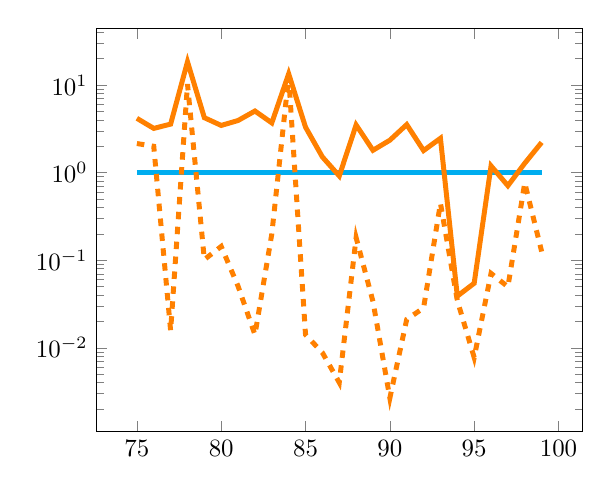
\begin{tikzpicture}[scale=0.9]
\begin{semilogyaxis}
\addplot[color=cyan,line width=2pt,mark options={solid}] coordinates {(75,1.0)(76,1.0)(77,1.0)(78,1.0)(79,1.0)(80,1.0)(81,1.0)(82,1.0)(83,1.0)(84,1.0)(85,1.0)(86,1.0)(87,1.0)(88,1.0)(89,1.0)(90,1.0)(91,1.0)(92,1.0)(93,1.0)(94,1.0)(95,1.0)(96,1.0)(97,1.0)(98,1.0)(99,1.0)};
\addplot[color=orange,line width=2pt,mark options={solid}] coordinates {(75,4.167640863097981)(76,3.198910330362423)(77,3.5794013025185327)(78,18.427774718667617)(79,4.239653379947609)(80,3.4576133137441367)(81,3.937602224654697)(82,5.051131322134538)(83,3.6979255310444143)(84,13.42241389209162)(85,3.3010698901548197)(86,1.5099395199226504)(87,0.9166133922819582)(88,3.503141167962537)(89,1.8004826646595617)(90,2.345443688236125)(91,3.534787234487251)(92,1.7869888170868897)(93,2.4656138208598115)(94,0.0388982293351494)(95,0.054531167751237786)(96,1.1928677160353975)(97,0.7086699154336324)(98,1.2799201661706583)(99,2.2114197806956057)};
\addplot[dashed,color=orange,line width=2pt,mark options={solid}] coordinates {(75,2.1491104106771814)(76,1.9987436978168398)(77,0.01569586341211839)(78,10.27613008842737)(79,0.1016813623505798)(80,0.14363539679208187)(81,0.050449401333145544)(82,0.014100487488133081)(83,0.19995404780961845)(84,12.550560375270152)(85,0.014104298089881706)(86,0.0087944100818767)(87,0.004010090780165804)(88,0.18068945325291566)(89,0.033727000094619805)(90,0.0026684216223300397)(91,0.021113757427773615)(92,0.028485007439162078)(93,0.4473795184673021)(94,0.034724882475904016)(95,0.007756932678074836)(96,0.07067214448300808)(97,0.04969262409917228)(98,0.766226563190781)(99,0.12561437184548097)};

\end{semilogyaxis}
\end{tikzpicture}
